\chapter{Arhitektura i dizajn sustava}
		
			Arhitektura sustava je web aplikacija kojoj će korisnici pristupati pomoću web preglednika. Odlučili smo se na takvu arhitekturu jer je cilj sustava da bude što jednostavniji za korištenje i da mu se može pristupiti sa svih mjesta.
			
			\begin{figure}[H]
				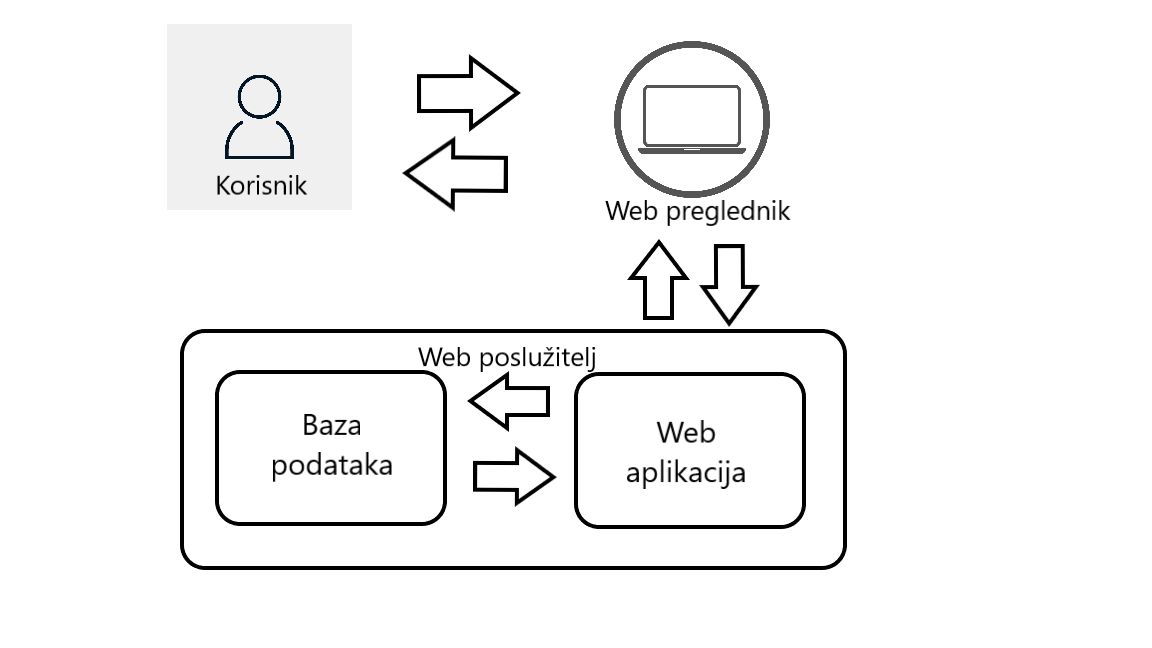
\includegraphics[scale=0.4]{slike/Skica_sustava.png} %veličina slike u odnosu na originalnu datoteku i pozicija slike
				\centering
				\caption{Skica sustava}
				\label{fig:sustav}
			\end{figure}
			
			Programski jezik koji smo odabralni za izradu aplikacije je java s razvojnim okvirom Spring Boot te javaScript. Odabrano razvojno okruženje je IntelliJ IDEA. 
			Aplikacija je organizirana u dva sloja: frontend i backend. Za izradu frontenda koristi se React. Frontend i backend komuniciraju pomoću RESTa. Backend se sastoji od tri sloja:
		\begin{itemize}
		\item Kontroler - služi za komunikaciju s frontendom. Zaprima HTTP zathtjev te određuje koja će se funkcionalnost izvršavati
		\item Servis - u njima se odvijaju poslovne logike i sve funkcionalnosti aplikacije
		\item Repozitorij - dohvaća i sprema podatke u bazu podataka
	\end{itemize}

\begin{figure}[H]
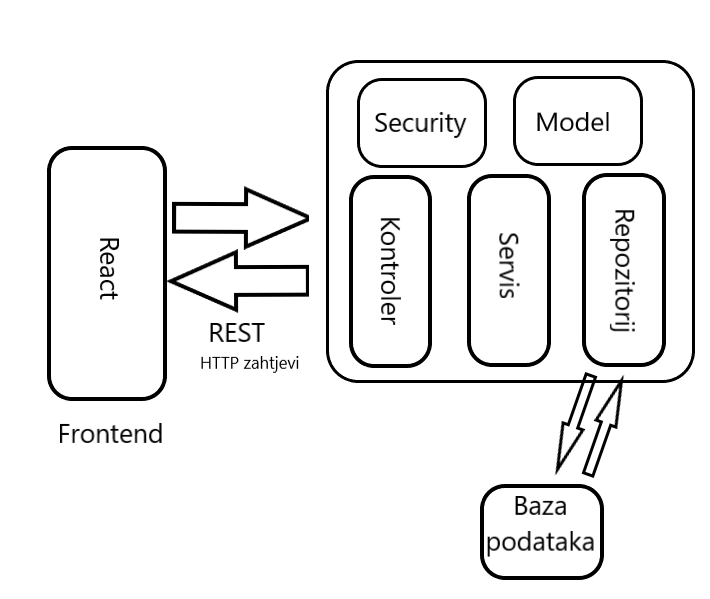
\includegraphics[scale=0.4]{slike/Skica_aplikacije.png} %veličina slike u odnosu na originalnu datoteku i pozicija slike
\centering
\caption{Skica aplikacije}
\label{fig:aplikacija}
\end{figure}


	
		

		

				
		\section{Baza podataka}
			
		Za potrebe sustava za zamjenu soba koristit ćemo relacijsku bazu podataka koja nam omogućuje oblikovanje objekata iz stvarnog svijeta pomoću povezanih tablica - relacija. Svaka je tablica definirana vlastitim nazivom i skupom različitih atributa koji je opisuju. Glavna je zadaća baze podataka pohrana, brzo pronalaženje i dohvaćanje te dodavanje i brisanje podataka. Baza podataka ovog sustava sastoji se od entiteta:
		\begin{itemize}
			\item Student
			\item Oglas
			\item Soba
			\item Grad
			\item Dom
			\item Paviljon
			\item StudentskiCentar
			\item Obavijest
			\item Zaposlenik SC
			\item TrazeniUvjeti
			\item Lajkovi
			\item StudentObavijesti
			
		\end{itemize}
		
			\subsection{Opis tablica}
			

			\textbf{Student } Entitet sadrži informacije o korisniku aplikacije - studentu. Sadrži sljedeće atribute: identifikator studenta, korisničko ime, ime, prezime, e-mail adresu, JMBAG, lozinku te oznaku za primanje mailova. Entitet je u vezi \textit{Many-to-Many} s entitetom Obavijest preko identifikatora obavijesti, u vezi \textit{One-to-One} s entitetom Oglas preko atributa statusa oglasa, u vezi \textit{One-to-One} s entitetom TrazeniUvjeti preko atributa identifikatora uvjeta te u vezi \textit{One-to-One} s entitetom Oglas. 
				
				
				
				\begin{longtabu} to \textwidth {|X[6, 2]|X[6, 2]|X[20, l]|}
					
					\hline \multicolumn{3}{|c|}{\textbf{Student}}	 \\[3pt] \hline
					\endfirsthead
					
					\hline \multicolumn{3}{|c|}{\textbf{Student}}	 \\[3pt] \hline
					\endhead
					
					\hline 
					\endlastfoot
					
					\textbf{idKorisnik} & UUID	& jedinstveni identifikator studenta (korisnika) 	\\ \hline
					korisnickoIme	& VARCHAR & jedinstveno korisničko ime  	\\ \hline 
					jmbag & VARCHAR & jedinstveni JMBAG studenta \\ \hline 
					ime & VARCHAR & ime studenta 		\\ \hline
					prezime & VARCHAR & prezime studenta \\ \hline
					email & VARCHAR & e-mail adresa studenta \\ \hline
					hashLozinke & VARCHAR & hash lozinka \\ \hline
					obavijestiNaMail & BOOLEAN & oznaka želi li student primati obavijesti na mail \\ \hline
					viseOvlasti & BOOLEAN & aa \\ \hline
					\textit{idStatusOglasa} & BOOLEAN & oznaka potvrde \\ \hline
					\textit{idTrazeniUvjeti} & VARCHAR & traženi kriteriji za sobu za zamjenu \\ \hline
				 
					
				\end{longtabu}
			
				\textbf{Oglas } Entitet sadrži informacije koje su vezane uz oglas koji student predaje. Sadrži atribute: ID oglasa, naslov oglasa, opis te datum objave oglasa. Entitet je u vezi \textit{One-to-One} s entitetom Status preko atributa identifiaktora statusa oglasa i u vezi \textit{One-to-Many} s entitetom Obavijest preko atributa identifikatora oglasa.
			
				\begin{longtabu} to \textwidth {|X[6, 2]|X[6, 2]|X[20, l]|}
					
					\hline \multicolumn{3}{|c|}{\textbf{Oglas}}	 \\[3pt] \hline
					\endfirsthead
					
					\hline \multicolumn{3}{|c|}{\textbf{Oglas}}	 \\[3pt] \hline
					\endhead
					
					\hline 
					\endlastfoot
					
					\textbf{idOglas} & UUID	& jedinstveni identifikator oglasa 	\\ \hline
					naslov	& VARCHAR & naslov oglasa  	\\ \hline 
					opis & VARCHAR & opis oglasa \\ \hline 
					objavljen & DATE & datum objavljivanja oglasa 		\\ \hline
					godina & INTEGER & godina objavljivanja oglasa \\ \hline
					\textit{idStatusOglasa} & VARCHAR & status oglasa \\ \hline
					
					 
					
					
				\end{longtabu}
			
				\textbf{Soba } Entitet sadrži informacije o sobi u studentskom domu. Sadrži atribute: broj sobe, kat na kojemu se soba nalazi,broj kreveta i vrstu kupaonice koja pripada sobi, kategoriju te identifikator paviljona i doma. Entitet je u vezi \textit{Many-to-One} s entitetom Paviljon preko atributa identifikatora paviljona i doma.
			
				\begin{longtabu} to \textwidth {|X[6, 2]|X[6, 2]|X[20, l]|}
					
					\hline \multicolumn{3}{|c|}{\textbf{Soba}}	 \\[3pt] \hline
					\endfirsthead
					
					\hline \multicolumn{3}{|c|}{\textbf{Soba}}	 \\[3pt] \hline
					\endhead
					
					\hline 
					\endlastfoot
					
					\textbf{broj} & INTEGER & broj sobe 	\\ \hline
					\textbf{kat} & INTEGER & kat na kojemu se soba nalazi \\ \hline 
					brojKreveta & VARCHAR & broj kreveta u sobi \\ \hline
					tipKupaonice & VARCHAR & vrsta dostupne kupaonice \\ \hline
					kategorija & VARCHAR & kategorija sobe \\ \hline
					\textbf{\textit{idPaviljon}} & UUID & identifikator paviljona kojemu soba pripada \\ \hline
					\textbf{\textit{idDom}} & UUID & identifikator doma kojemu soba pripada \\ \hline
					
					
				\end{longtabu}
			
				\textbf{Grad } Entitet sadrži informacije o pojedinom gradu. Sadrži atribute: identifikator grada i naziv te identifikator studentskog centra tog grada. Entitet je u vezi \textit{One-To-One} s entitetom Studentski Centar preko atributa identifikatora studentskog centra i u vezi \textit{One-to-Many} s entitetom Dom preko identifikatora grada. 
			
				\begin{longtabu} to \textwidth {|X[6, 2]|X[6, 2]|X[20, l]|}
					
					\hline \multicolumn{3}{|c|}{\textbf{Grad}}	 \\[3pt] \hline
					\endfirsthead
					
					\hline \multicolumn{3}{|c|}{\textbf{Grad}}	 \\[3pt] \hline
					\endhead
					
					\hline 
					\endlastfoot
					
					\textbf{idGrad} & UUID	& jedinstveni identifikator grada	\\ \hline
					naziv	& VARCHAR & ime grada  	\\ \hline  
					\textit{idSc} & UUID & identifikator gradskog studentskog centra \\ \hline
					
					
				\end{longtabu}
			
				\textbf{Dom } Entitet sadrži sve važne informacije o pojedinom studentskom domu. Sadrži atribute: ID doma, naziv doma, ID grada u kojemu se dom nalazi te oznaku ima li dom vlastitu menzu. Entitet je u vezi \textit{Many-to-One} s entitetom Grad preko atributa identifikatora grada i u vezi \text{One-To-Many} s entitetom Paviljon preko identifikatora doma. 
			
				\begin{longtabu} to \textwidth {|X[6, 2]|X[6, 2]|X[20, l]|}
					
					\hline \multicolumn{3}{|c|}{\textbf{Dom}}	 \\[3pt] \hline
					\endfirsthead
					
					\hline \multicolumn{3}{|c|}{\textbf{Dom}}	 \\[3pt] \hline
					\endhead
					
					\hline 
					\endlastfoot
					
					\textbf{idDom} & UUID	& jedinstveni identifikator studentskog doma 	\\ \hline
					naziv	& VARCHAR & ime studentskog doma  	\\ \hline 
					imaMenzu & BOOLEAN & oznaka ima li dom vlastitu menzu \\ \hline
					\textit{idGrad} & UUID & identifikator grada u kojemu se dom nalazi \\ \hline
					
					
				\end{longtabu}
			
				\textbf{Paviljon } Entitet sadrži sve informacije o pojedinom paviljonu studentskog doma. Sadrži atribute: identifikator paviljona, naziv te identifikator doma. Entitet je u vezi \textit{Many-to-One} s entitetom Dom preko atributa identifikatora doma te u vezi \textit{One-to-Many} s entitetom Soba preko indetifikatora paviljona. 
			
				\begin{longtabu} to \textwidth {|X[6, 2]|X[6, 2]|X[20, l]|}
					
					\hline \multicolumn{3}{|c|}{\textbf{Paviljon}}	 \\[3pt] \hline
					\endfirsthead
					
					\hline \multicolumn{3}{|c|}{\textbf{Paviljon}}	 \\[3pt] \hline
					\endhead
					
					\hline 
					\endlastfoot
					
					\textbf{idPaviljon} & UUID	& jedinstveni identifikator paviljona	\\ \hline
					naziv & VARCHAR & naziv paviljona  	\\ \hline 
					\textit{idDom} & UUID & identifikator doma u kojemu se paviljon nalazi \\ \hline
					
					
				\end{longtabu}
			
			
				\textbf{Studentski centar } Entitet sadrži informacije o studentskom centru. Sadrži atribute: identifikator studentskog centra, naziv te identifikator grada u kojemu se studentski centar nalazi. Entitet je u vezi \textit{One-to-One} s entitetom Grad preko atributa identifikatora grada te u vezi \textit{One-to-Many} s entitetom Zaposlenik SC preko identifikatora studentskog centra. 
			
				\begin{longtabu} to \textwidth {|X[6, 2]|X[6, 2]|X[20, l]|}
					
					\hline \multicolumn{3}{|c|}{\textbf{Studentski Centar}}	 \\[3pt] \hline
					\endfirsthead
					
					\hline \multicolumn{3}{|c|}{\textbf{Studentski centar}}	 \\[3pt] \hline
					\endhead
					
					\hline 
					\endlastfoot
					
					\textbf{idSc} & UUID & jedinstveni identifikator studentskog centra	\\ \hline
					naziv  & VARCHAR & ime studentskog centra  	\\ \hline
					\textit{idGrad} & UUID & identifikator grada u kojemu se nalazi studentski centar \\ \hline
					
					
				\end{longtabu}
			
				\textbf{Obavijest} Entitet sadrži informacije o obavijestima koje aplikacija šalje studentima. Sadrži entitete: identifikator obavijesti, tekst, oznaku je li obavijest procitana, vrijeme slanja obavijesti te listu studenata kojima se obavijest šalje i identifikator oglasa za koji se obavijest šalje. Entitet je u vezi \textit{Many-to-Many} s entitetom Student te u vezi \textit{Many-to-One} s entitetom Oglas preko identifikatora oglasa. 
			 
				\begin{longtabu} to \textwidth {|X[6, 2]|X[6, 2]|X[20, l]|}
					
					\hline \multicolumn{3}{|c|}{\textbf{Obavijest}}	 \\[3pt] \hline
					\endfirsthead
					
					\hline \multicolumn{3}{|c|}{\textbf{Obavijest}}	 \\[3pt] \hline
					\endhead
					
					\hline 
					\endlastfoot
					
					\textbf{idObavijest} & UUID & jedinstveni identifikator obavijesti	\\ \hline
					tekst  & VARCHAR & tekst obavijesti  	\\ \hline 
					procitana & BOOLEAN & oznaka je li poruka pročitana \\ \hline
					vrijeme & DATE & vrijeme slanja obavijesti \\ \hline
					\textit{idOglas} & UUID & identifikator oglasa za koji se obavijest generira \\ \hline
					
					
				\end{longtabu}
			
				\textbf{Zaposlenik SC } Entitet sadrži informacije o zaposleniku u studentskom centru. Sadrži atribute: identifikator zaposlenika, korisničko ime i lozinku za prijavu u sustav, ime i prezime zaposlenika, e-mail adresu te identifikator studentskog centra u kojem je zaposlen.
			
				\begin{longtabu} to \textwidth {|X[6, 2]|X[6, 2]|X[20, l]|}
					
					\hline \multicolumn{3}{|c|}{\textbf{Zaposlenik SC}}	 \\[3pt] \hline
					\endfirsthead
					
					\hline \multicolumn{3}{|c|}{\textbf{Zaposlenik SC}}	 \\[3pt] \hline
					\endhead
					
					\hline 
					\endlastfoot
					
					\textbf{idZaposlenik} & UUID	& jedinstveni identifikator zaposlenika studentskog centra	\\ \hline
					korisnickoIme & VARCHAR & jedinstveno korisničko ime zaposlenika studentskog centra \\ \hline
					ime & VARCHAR & ime zaposlenika studentskog centra \\ \hline
					prezime & VARCHAR & prezime zaposlenika studentskog centra \\ \hline
					email & VARCHAR & e-mail adresa zaposlenika studentskog centra \\ \hline
					hashLozinke & VARCHAR & hash lozinke \\ \hline
					\textit{idSc} & UUID & identifikator studentskog centra u kojemu je zaposlen \\ \hline
				
					
					
				\end{longtabu}
			
				\begin{longtabu} to \textwidth {|X[6, 2]|X[6, 2]|X[20, l]|}
					
					\hline \multicolumn{3}{|c|}{\textbf{TrazeniUvjeti}}	 \\[3pt] \hline
					\endfirsthead
					
					\hline \multicolumn{3}{|c|}{\textbf{TrazeniUvjeti}}	 \\[3pt] \hline
					\endhead
					
					\hline 
					\endlastfoot
					
					\textbf{idTrazeniUvjeti} & UUID	& jedinstveni identifikator skupa traženih uvjeta	\\ \hline
					brojKreveta & VARCHAR & traženi broj kreveta \\ \hline
					tipKupaonice & VARCHAR & traženi tip kupaonice \\ \hline
					kateogrija & VARCHAR & tražena kategorija \\ \hline
					godina & INTEGER & godina za koju se predaje oglas \\ \hline
					komentar & VARCHAR & dodatni komentari vezani uz tražene uvjete \\ \hline
					
					
					
					
					
				\end{longtabu}
			
				\textbf{Lajkovi} Entitet sadrži informacije vezane uz 'lajkove' oglasa. Sadrži atribute: identifikator oglasa i identifikator studenta te ocjenu. Entitet je u vezi \textit{Many-to-One} s entitetom Student preko identifikatora studenta i u vezi \textit{Many-to-One} s entitetom Oglas preko identifikatora oglasa.
			
				\begin{longtabu} to \textwidth {|X[6, 2]|X[6, 2]|X[20, l]|}
					
					\hline \multicolumn{3}{|c|}{\textbf{Lajkovi}}	 \\[3pt] \hline
					\endfirsthead
					
					\hline \multicolumn{3}{|c|}{\textbf{Lajkovi}}	 \\[3pt] \hline
					\endhead
					
					\hline 
					\endlastfoot
					
					\textbf{idOglas} & UUID & jedinstveni identifikator oglasa koji se ocjenjuje \\ \hline
					\textbf{idStudent} & UUID & jedinstveni identifikator studenta koji je 'dao lajk' \\ \hline
					ocjena & INTEGER & iznos ocjene \\ \hline
					
					
				\end{longtabu}
			
				\begin{longtabu} to \textwidth {|X[6, 2]|X[6, 2]|X[20, l]|}
					
					\hline \multicolumn{3}{|c|}{\textbf{Status oglasa}}	 \\[3pt] \hline
					\endfirsthead
					
					\hline \multicolumn{3}{|c|}{\textbf{Status oglasa}}	 \\[3pt] \hline
					\endhead
					
					\hline 
					\endlastfoot
					
					\textbf{idStautsOglasa} & UUID & jedinstveni identifikator statusa oglasa \\ \hline
					status & INTEGER & aa \\ \hline
					\textit{idOglas} & UUID & identifikator oglasa\\ \hline
					\textit{idStudent} & UUID & identifikator studenta \\ \hline
					
					
					
					
				\end{longtabu}
			
				\begin{longtabu} to \textwidth {|X[6, 2]|X[6, 2]|X[20, l]|}
					
					\hline \multicolumn{3}{|c|}{\textbf{StudentObavijesti}}	 \\[3pt] \hline
					\endfirsthead
					
					\hline \multicolumn{3}{|c|}{\textbf{StudentObavijesti}}	 \\[3pt] \hline
					\endhead
					
					\hline 
					\endlastfoot
					
					\textit{studentiIdKorisnik} & UUID & aa \\ \hline
					\textit{obavijestiIdObavijest} & UUID & aa \\ \hline
					
					
					
					
				\end{longtabu}
			
				\begin{longtabu} to \textwidth {|X[6, 2]|X[6, 2]|X[20, l]|}
					
					\hline \multicolumn{3}{|c|}{\textbf{Broj kreveta}}	 \\[3pt] \hline
					\endfirsthead
					
					\hline \multicolumn{3}{|c|}{\textbf{Broj kreveta}}	 \\[3pt] \hline
					\endhead
					
					\hline 
					\endlastfoot
					
					
					
					
				\end{longtabu}
			
				\begin{longtabu} to \textwidth {|X[6, 2]|X[6, 2]|X[20, l]|}
					
					\hline \multicolumn{3}{|c|}{\textbf{Oznake kategorija}}	 \\[3pt] \hline
					\endfirsthead
					
					\hline \multicolumn{3}{|c|}{\textbf{Oznake kategorija}}	 \\[3pt] \hline
					\endhead
					
					\hline 
					\endlastfoot
					
					
					
				\end{longtabu}
			
				\begin{longtabu} to \textwidth {|X[6, 2]|X[6, 2]|X[20, l]|}
					
					\hline \multicolumn{3}{|c|}{\textbf{Tip kupaonice}}	 \\[3pt] \hline
					\endfirsthead
					
					\hline \multicolumn{3}{|c|}{\textbf{Tip kupaonice}}	 \\[3pt] \hline
					\endhead
					
					\hline 
					\endlastfoot
					
					
					
					
				\end{longtabu}
		
		
			
			
			\subsection{Dijagram baze podataka}
				\begin{figure}[H]
					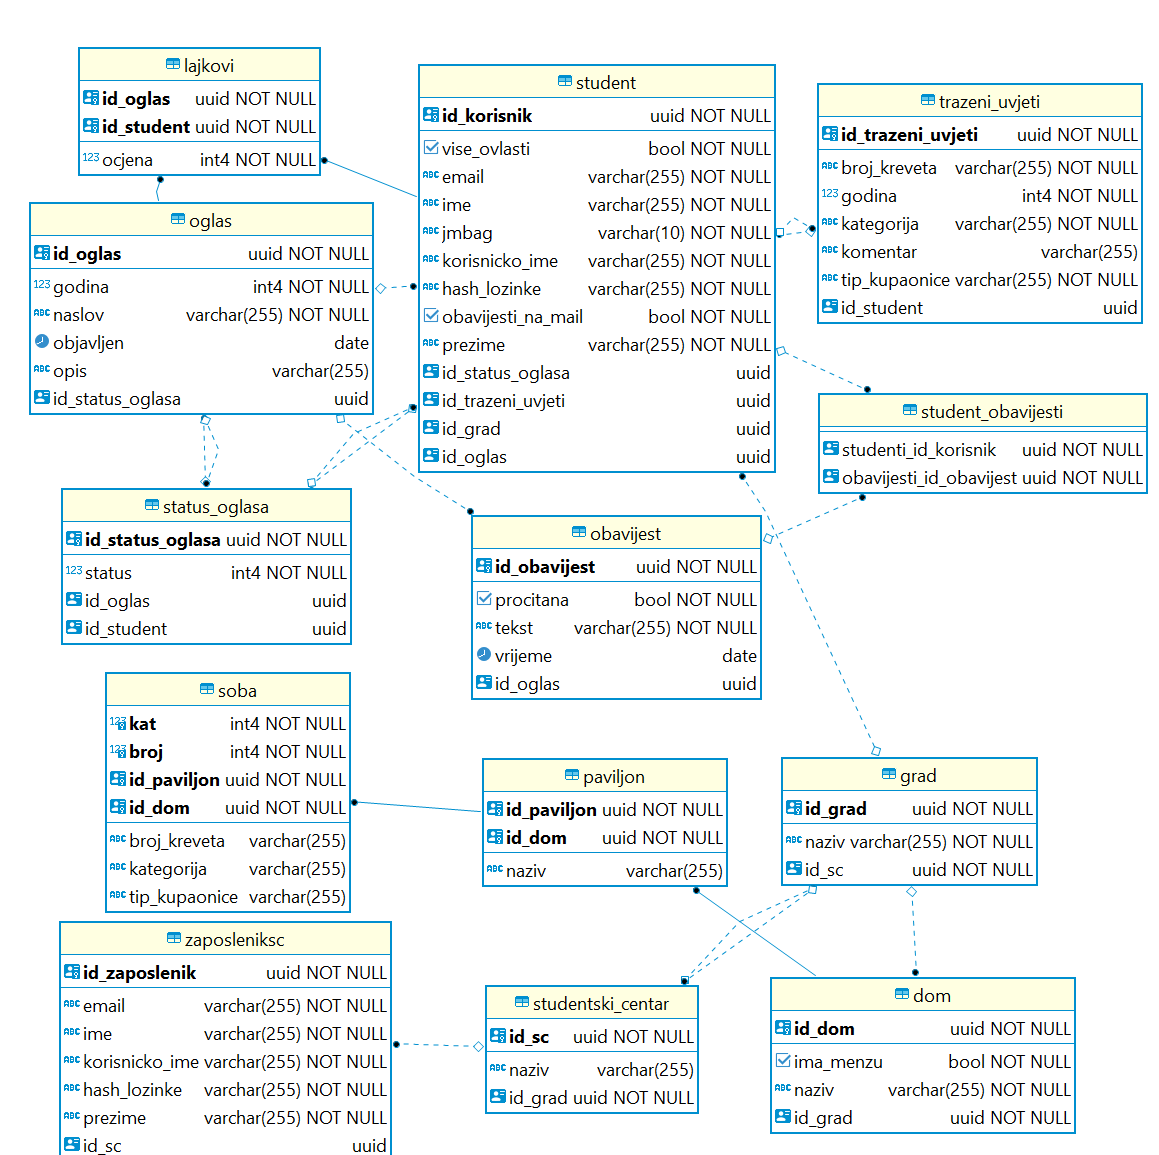
\includegraphics[scale=0.4]{dijagrami/ERdijagram.png} %veličina slike u odnosu na originalnu datoteku i pozicija slike
					\centering
					\caption{ER dijagram baze podataka}
					\label{fig:er}
				\end{figure}
			
			\eject
			
			
		\section{Dijagram razreda}
		
			\textit{Potrebno je priložiti dijagram razreda s pripadajućim opisom. Zbog preglednosti je moguće dijagram razlomiti na više njih, ali moraju biti grupirani prema sličnim razinama apstrakcije i srodnim funkcionalnostima.}\\
			
			\textbf{\textit{dio 1. revizije}}\\
			
			\textit{Prilikom prve predaje projekta, potrebno je priložiti potpuno razrađen dijagram razreda vezan uz \textbf{generičku funkcionalnost} sustava. Ostale funkcionalnosti trebaju biti idejno razrađene u dijagramu sa sljedećim komponentama: nazivi razreda, nazivi metoda i vrste pristupa metodama (npr. javni, zaštićeni), nazivi atributa razreda, veze i odnosi između razreda.}\\
			
			\textbf{\textit{dio 2. revizije}}\\			
			
			\textit{Prilikom druge predaje projekta dijagram razreda i opisi moraju odgovarati stvarnom stanju implementacije}
			
			
			
			\eject
		
		\section{Dijagram stanja}
			
			
			\textbf{\textit{dio 2. revizije}}\\
			
			\textit{Potrebno je priložiti dijagram stanja i opisati ga. Dovoljan je jedan dijagram stanja koji prikazuje \textbf{značajan dio funkcionalnosti} sustava. Na primjer, stanja korisničkog sučelja i tijek korištenja neke ključne funkcionalnosti jesu značajan dio sustava, a registracija i prijava nisu. }
			
			
			\eject 
		
		\section{Dijagram aktivnosti}
			
			\textbf{\textit{dio 2. revizije}}\\
			
			 \textit{Potrebno je priložiti dijagram aktivnosti s pripadajućim opisom. Dijagram aktivnosti treba prikazivati značajan dio sustava.}
			
			\eject
		\section{Dijagram komponenti}
		
			\textbf{\textit{dio 2. revizije}}\\
		
			 \textit{Potrebno je priložiti dijagram komponenti s pripadajućim opisom. Dijagram komponenti treba prikazivati strukturu cijele aplikacije.}